\section{Background and Motivation} 
\label{sec:motivation}

\subsection{The General Smith-Waterman (S-W) Algorithm}
\label{subsec:general_SW}

As a fundamental operation in computational genetics, 
the acceleration of the general S-W algorithm has attracted a large amount of attention from academia \cite{Aluru2014}. 
The general S-W algorithm is anti-diagonal parallelizable, 
since the elements along each anti-diagonal in the S-W matrix are independent of each other, 
and each element only depends on three elements from the previous two anti-diagonals \cite{Edmiston1988}. 
Therefore, the wavefront property, as illustrated in Figure \ref{fig:F3C2}, 
has been used by researchers in almost all kinds of platforms for the S-W algorithm acceleration \cite{Wozniak1997}\cite{Arram2013}\cite{Preusser2012}\cite{Olson2012}\cite{RaceLogic}.
%REF achieves significant speedup with the anti-diagonal parallelism well-explored.
\begin{figure}[!hbt]
	\begin{center}
		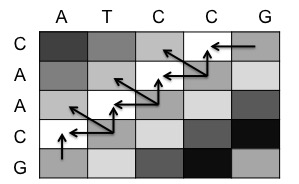
\includegraphics[width=1.8in]{Figures/Figure3C2.jpg}
		\caption {The anti-diagonal parallelism explored in the general S-W algorithm.}
		\label{fig:F3C2}
	\end{center}
\end{figure}

\subsection{S-W in BWA-MEM: An Extended S-W Algorithm} 
\label{subsec:Smith-Waterman}
In the NGS flow, a chemical sequencer chops many copies of a human genome into small segments and determines their nucleotide sequences. 
A small segment is called a read, which is generally composed of hundreds of nucleotides. 
We use the term ``base-pair'' (bp) as the unit of nucleotide. %for the rest of discussion.
Meanwhile, a pre-existing human genome is used as a reference with 3.2 billions bps \cite{Mardis2008}.
Read alignment is naturally a string matching problem. %to find the mapping between a read and the reference.
To be specific, the goal is to find a gap-tolerant mapping, i.e. an inexact mapping, between the read and the reference, that maximizes the total alignment score. 
%with a given score function that enumerates all possible character mappings.

The S-W algorithm \cite{Smith1981} is the classic approach that addresses this problem. 
This dynamic programming algorithm tolerates an arbitrary number of mismatches and gaps, 
and is guaranteed to generate the optimal solution with the highest score. 
However, the time complexity is O($nm$), which is proportional to the length of the read ($m$) and the reference ($n$). 
For the human genome, $n$ is approximately 3.2 billions, 
which makes it prohibitive for processing all the billions of reads collected from an individual using the S-W algorithm.

An alternative solution proposed in \cite{BWA} is developed based on the backward search with the Burrows-Wheeler Transform (BWT).
%which performs extremely efficiently for exact string matching. 
%Two strings are considered as exactly matched to both of them are identical. 
With the BWT-encoded reference genome, this approach achieves O($m$) time for a read to find all exactly matched substrings in the reference genome, 
independent of the size of the long reference genome. For gap-tolerant matching using backward search, 
nevertheless, the complexity is exponential.

The state-of-the-art read aligners harness both and turn to a two-step heuristic method \cite{Heng2010}. 
First, a series of substrings of a read are selected and aligned to the reference genome without gaps, i.e. exact mappings, by using BWT-based algorithms.
%This step is fast and is achieved by using BWT-based algorithms.
After that, such short un-gapped alignments serve as seeds and extended both leftward and rightward using S-W algorithm. 
Extended segments in reads are usually called queries, and their corresponding segments in the reference genome are called targets. 
This paradigm, seed-and-extend, first introduced in the famous BLAST algorithm \cite{BLAST1990}, is deemed a milestone for read alignment.
Most of the contemporary read alignment algorithms, such as SOAP \cite{SOAP}, BFAST \cite{BFAST}, LAST \cite{LAST}, Bowtie 2 \cite{Bowtie2}, and BWA-MEM \cite{BWA-MEM}, 
are derived from this canonical paradigm.

The Burrows-Wheeler Aligner (BWA) is by far the most prevalent read alignment software package \cite{BWA}\cite{BWA-SW}\cite{BWA-MEM}.
BWA-MEM \cite{BWA-MEM} is the latest generation among BWA \cite{BWA}, BWA-SW \cite{BWA-SW}, and BWA-MEM \cite{BWA-MEM}. 
BWA-MEM demonstrates better performance than several state-of-the-art tools 
and is also adaptable to a wide range of read lengths from 70bp to a few millions bps. 
The algorithm falls into the seed-and-extend category, but introduces two innovations.

First, unlike BLAST \cite{BLAST1990}, whose seed length is fixed, BWA-MEM adopts the super maximal exact matches (SMEM) method \cite{Heng2012} to generate
a group of variable-length substrings from a read as seeds; this is demonstrated in Figure \ref{fig:F1C2}. 
%a maximum exact match (MEM) is an exact string match that cannot be extended leftwards or rightwards to obtain a longer exact match, 
%and an SMEM is a MEM that is not contained in other MEMs on the read. 
An SMEM can possibly start from any location of a read and its length ranges from one to the length of a read ($m$). 
This feature results in a sharp variation of the seed lengths, which makes the sizes of inputs of the S-W algorithm vary substantially in BWA-MEM.
%BWA-MEM uses an algorithm proposed in \cite{Heng2012} to find the set of SMEMs as seeds for Smith-Waterman extension. 
%The algorithm is derived from the classic BWT-based backward search algorithm with linear time complexity, which is relatively fast compared to the quadratic Smith-Waterman extension.

\begin{figure}[!hbt]
	\begin{center}
		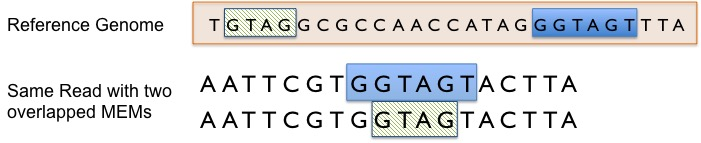
\includegraphics[width=3.2in]{Figures/Figure1C2.jpg}
		\caption {A maximal exact match (MEM) is an exact match that cannot be extended leftward or rightward without introducing a mismatch. Both of the matches illustrated are MEMs. An SMEM is a MEM that is not contained in other MEMs on the read. In this case, the longer match fully covers the shorter one on the read, and is not fully covered by any other MEM. Therefore, the longer match is an SMEM, but the shorter one is not.}
		\label{fig:F1C2}
	\end{center}
\end{figure}

%Second, as achieves the highest time complexity among all the main steps of BWA-MEM, seed extension becomes the bottleneck the whole BWA-MEM algorithm. Like other seed-and-extend algorithms, BWA-MEM adopts Smith-Waterman, a quadratic time algorithm, for seed extension. 
Second, BWA-MEM does not use the standard S-W algorithm but further extends it to improve performance. 
In general, to align two strings of length $m$ and $n$, 
a $m$x$n$ score matrix is expected to be filled up so as to generate the highest score and its corresponding alignment. 
BWA-MEM, however, developed a pruning heuristic to eliminate the solution space \cite{BWA-MEM}.
When we calculate the score at reference position $x$ and query position $y$, BWA-MEM will stop extension 
if the difference between the best extension score and the score at ($x$, $y$) is larger than $Z+\lvert x-y \rvert \times p_{gapExt}$, 
where $p_{gapExt}$ is the gap extension penalty and $Z$ is an arbitrary cutoff \cite{BWA-MEM}.
Figure \ref{fig:F2C2} illustrates the impact of the pruning strategy on a 55x105 S-W input. 
Pruning saves more than half of the computation effort than does the standard S-W algorithm. 
This pruning heuristic performs even better when reads get longer, which is the trend of further NGS \cite{Mardis2008}\cite{Heng2010}\cite{BWA-MEM}.
However, none of the existing hardware acceleration techniques can be adopted easily and efficiently to accelerate the extended S-W algorithm. 
%As is described detailedly in \cite{BWA-MEM}, the customized Smith-Waterman will stop calculating the (i+1)-th and following columns in the score matrix if the highest score in the i-th column is way lower than the highest score known so far. Inside each column, meanwhile, only part of the score matrix elements are actually filled due to the existence of the pruning strategy. Figure \ref{fig:F2C2} illustrates the impact of the pruning strategy on a 55x105 score matrix. The two strings for alignment are 55bp and 105bp long respectively, and the standard Smith-Waterman algorithm should fill up a matrix with 5775 elements. Actually, only 2836 elements got calculated which means more than 50\% of the elements are pruned out in the BWA-MEM Smith-Waterman, meaning 2x speedup achieved.

\begin{figure}[!hbt]
	\begin{center}
		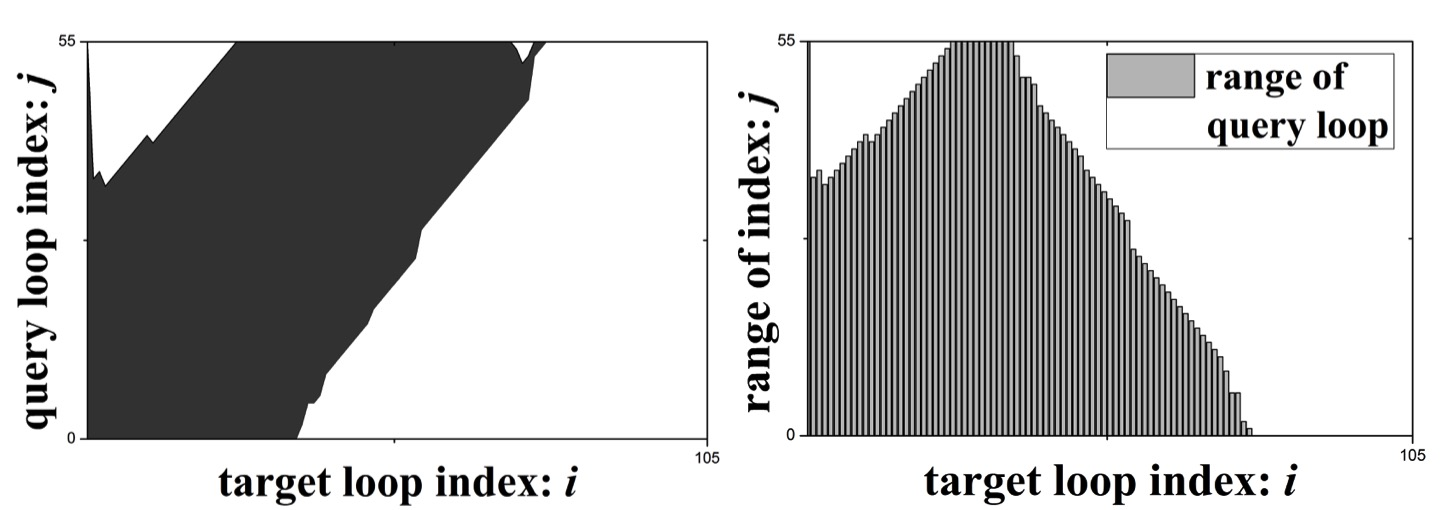
\includegraphics[width=3.2in]{Figures/Figure2C2.jpg}
		\caption {A 55x105 BWA-MEM Smith-Waterman task. The general S-W algorithm requires filling up a 55x105 matrix (5775 elements), but only 2836 elements (49\%) were actually filled with the help of pruning. The shaded area in the left graph illustrates the elements that got filled, and the right graph shows how many elements for each target loop index are actually calculated.}
		\label{fig:F2C2}
	\end{center}
\end{figure}

%The inefficiency of the wavefront-based technique will be discussed in the next section.

%\subsection{Inefficiencies of the Wavefront Technique in BWA-MEM} 
%\label{subsec:inefficiency}

%As a fundamental operation in computational genetics, the S-W algorithm has attracted a large amount attention from academia \cite{Aluru2014}. 
%The general S-W algorithm is inherently anti-diagonal parallelizable, 
%since the elements along each anti-diagonal in the S-W matrix are independent of each other, 
%and each element only depends on three elements from the previous two anti-diagonals \cite{Edmiston1988}. 
%Therefore, the wavefront property, as illustrated in Figure \ref{fig:F3C2}, 
%has been used by researchers in almost all kinds of platforms for the S-W algorithm acceleration \cite{Wozniak1997}\cite{Arram2013}\cite{Preusser2012}\cite{Olson2012}\cite{RaceLogic}.
%\begin{figure}[!hbt]
%	\begin{center}
%		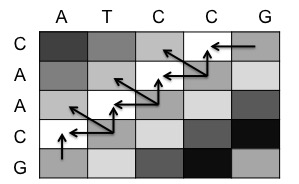
\includegraphics[width=1.8in]{Figures/Figure3C2.jpg}
%		\caption {Inherent anti-diagonal parallelism explored in S-W algorithm.}
%		\label{fig:F3C2}
%	\end{center}
%\end{figure}

%Nevertheless, tools such as BLAST \cite{BLAST1990} and BWA-MEM \cite{BWA-MEM} use the customized versions of the S-W algorithms.
%In BWA-MEM, we have three important observations that prevent us from using conventional wavefront technique for hardware acceleration.
%For simplicity of without lossing generality, 
%we abstract an acceleration platform to into a given number of unified processing elements (PEs) in the following discussions. 
%Each PE in the platform is capable to produce one DP computation per cycle to fill the score matrix. 
%A \textit{kernel} is composed of a group of PEs and can be assigned to execute one S-W task.
%We denote $m$x$n$ as a pair of input strings for S-W algorithm with length $m$ and $n$, respectively. 
%The maximum achievable degree of parallelism is bounded by the length of the shorter string.


